\paragraph{biguint-sub}

\subparagraph{Target}
Implement the substraction of two biguints.

\subparagraph{Constraints logic}
\begin{itemize}
    \item Equation for gate;
    \item Sumcheck for ouptput;
    \item Rangecheck for limbs.
\end{itemize}

\subparagraph{Circuit layout}
See \figref{fig:biguint-sub-circuit-layout}.
\begin{figure}[!ht]
    \centering
    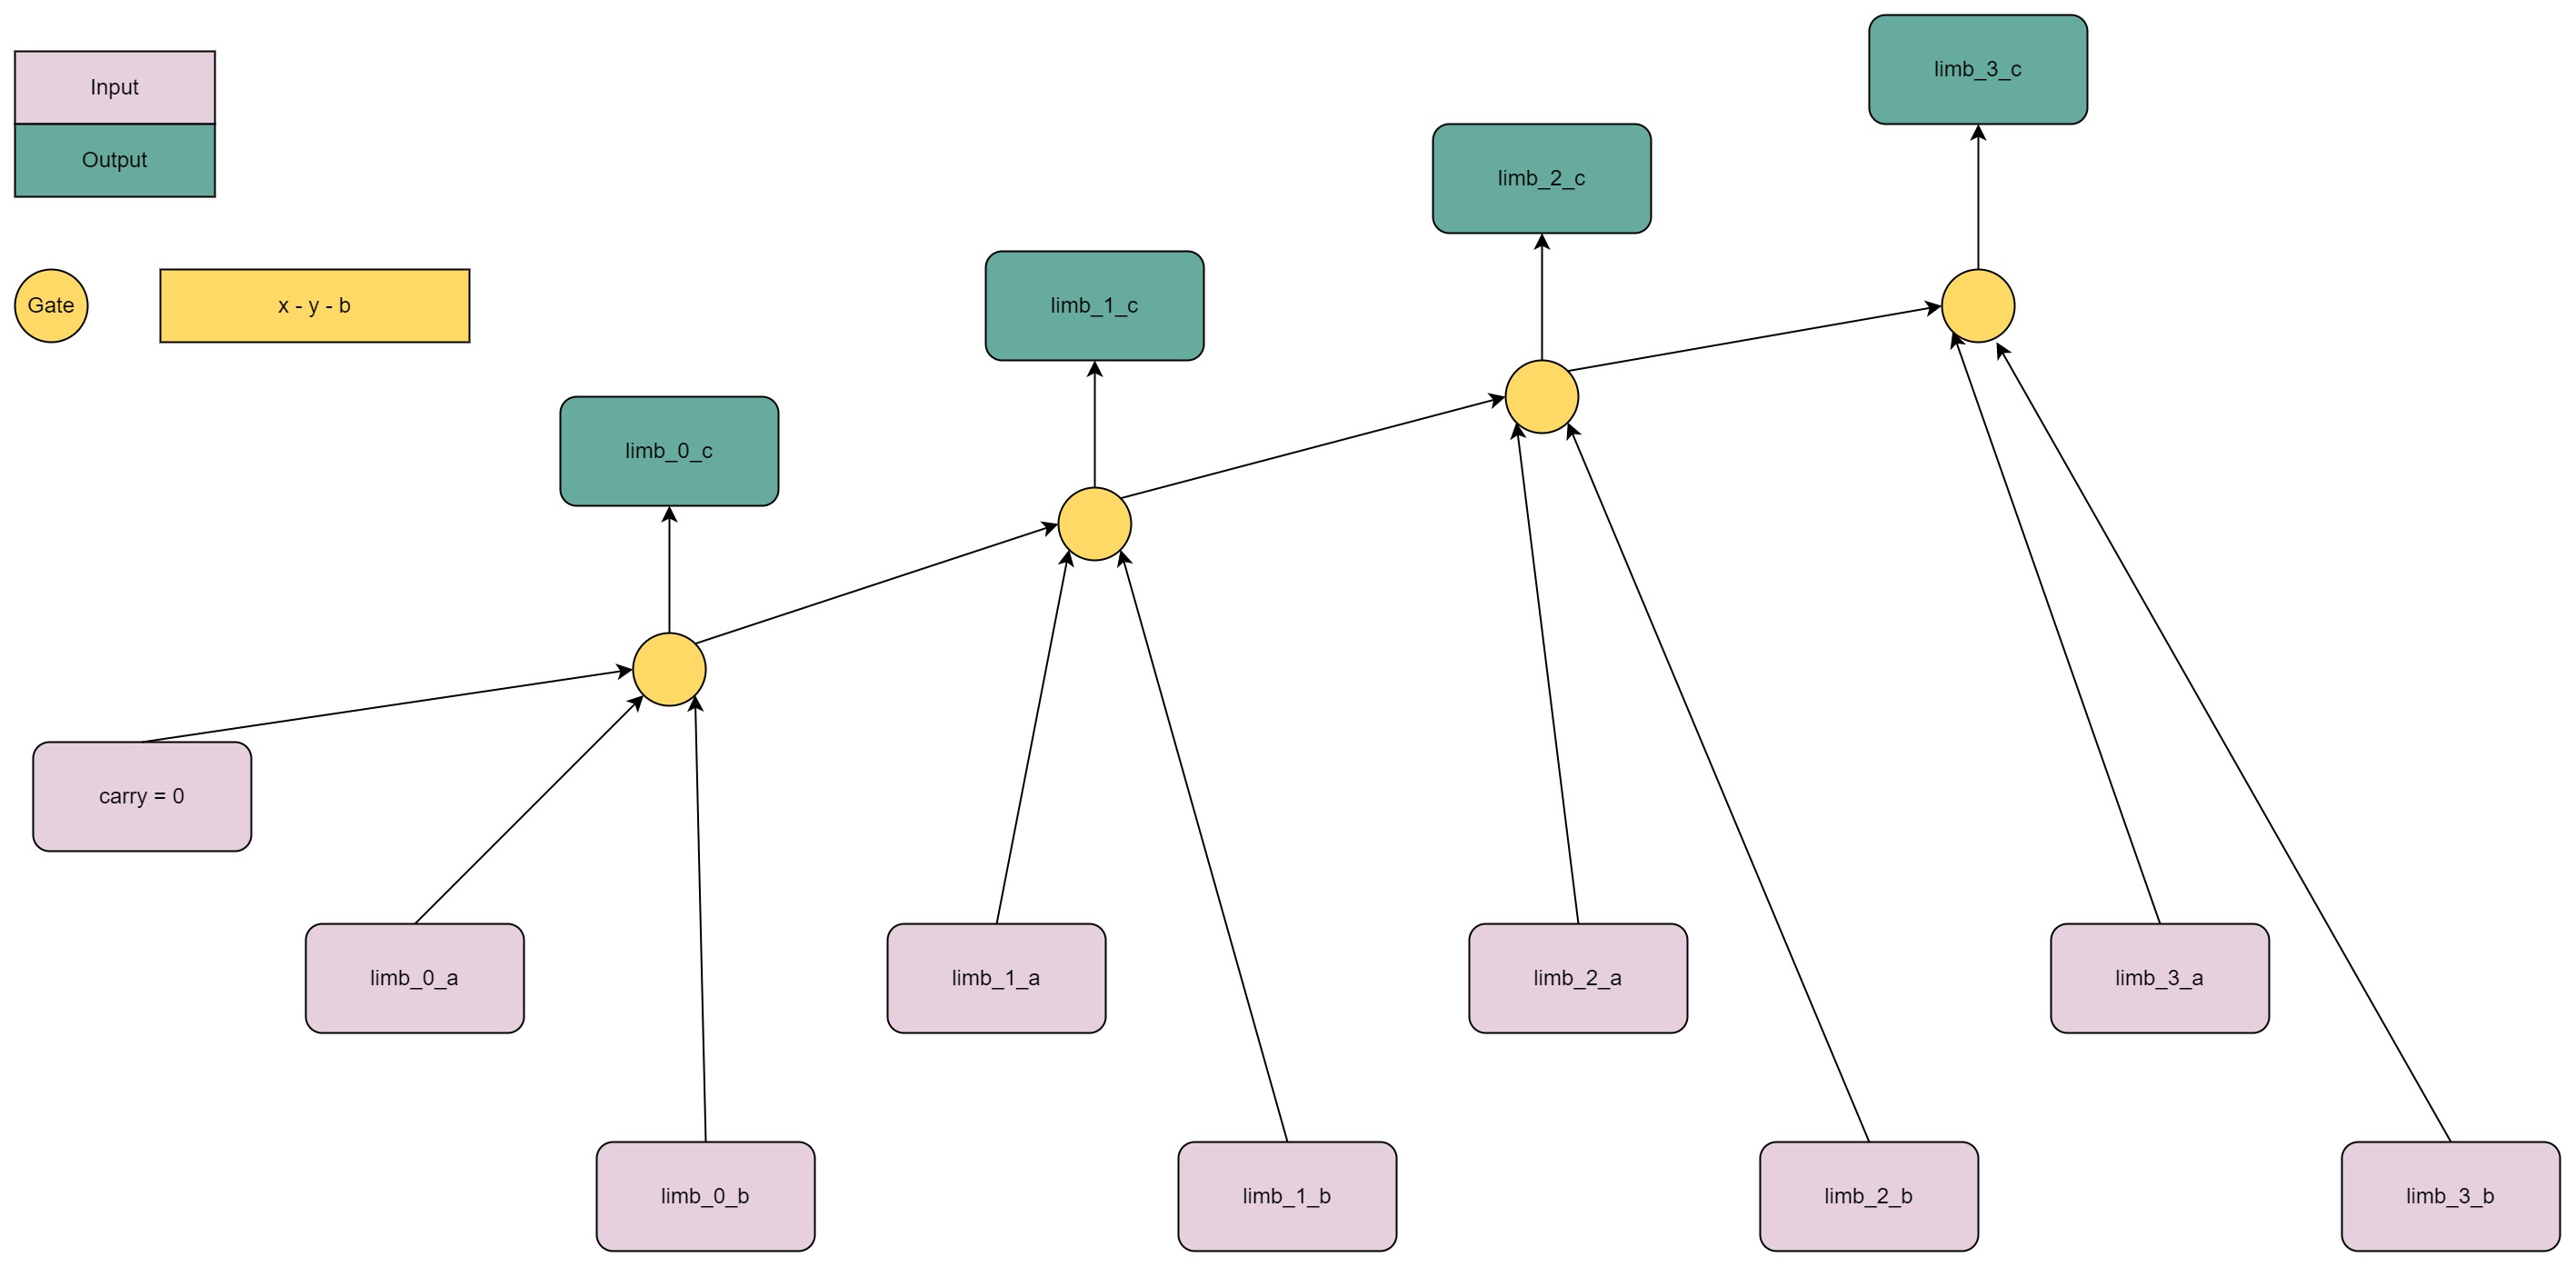
\includegraphics[width=0.8\textwidth]{biguint-sub-circuit-layout.jpg}
    \caption{biguint-sub circuit layout}
    \label{fig:biguint-sub-circuit-layout}
\end{figure}

\subparagraph{Trace layout}
See \figref{fig:biguint-sub-trace-layout}.
\begin{figure}[!ht]
    \centering
    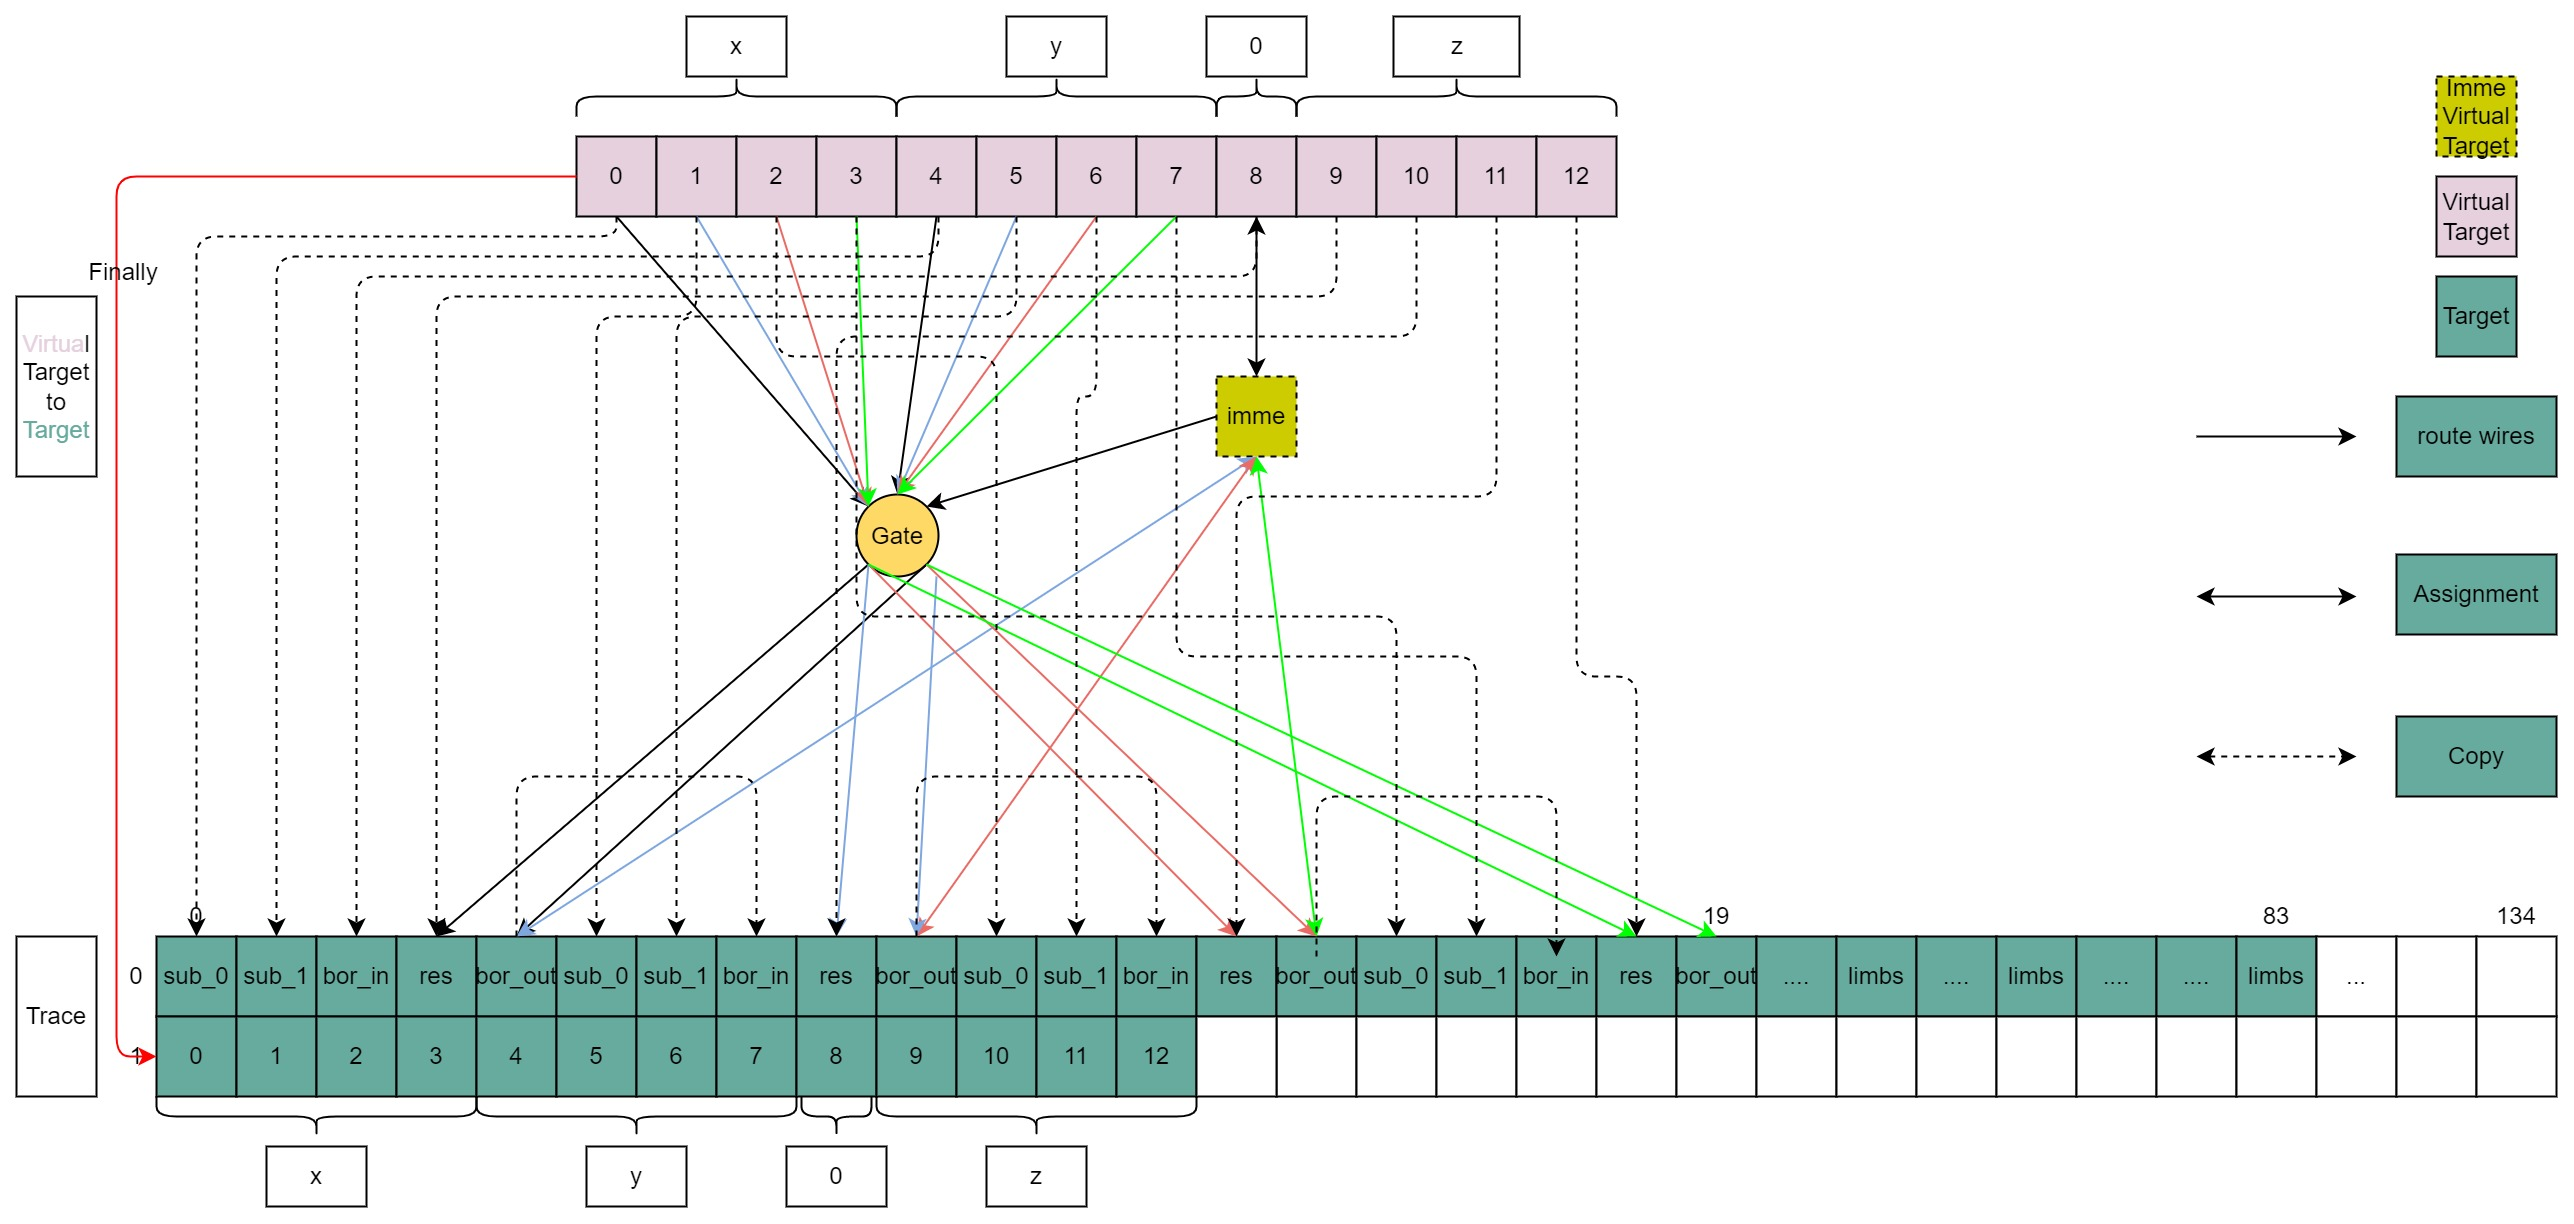
\includegraphics[width=0.8\textwidth]{biguint-sub-trace-layout.jpg}
    \caption{biguint-sub trace layout}
    \label{fig:biguint-sub-trace-layout}
\end{figure}

\subparagraph{Constraints info and costs}
\begin{itemize}
    \item constraints-num: $6 \times (3 + 32 / 2) = 114$
    \item copy-constraints: $16$
    \item max-degree: $4$
    \item wires-num: $6 \times (5 + 16) = 126$
\end{itemize}

\subparagraph{Questions}
\begin{itemize}
    \item Why not make rangecheck constraint for inputs?
    \item Could try to use the same constraint with add-gate.
\end{itemize}
